\section{Einführung}
\subsection{Maxwellsches Fallrad}
Das Maxwellsche Fallrad (auch bekannt als ``Jojo'') besteht aus einem Rad mit Schwerpunktsträgheitsmoment $J_S$, Masse $m$, um dessen horizontale Achse eine Schnur aufgewickelt ist. Diese ist an der Decke befestigt, sodass das Rad unter Einfluss der Schwerkraft nach unten gezogen wird. Dabei rollt sich die Schnur bis zur maximalen Fallhöhe $h_{\text{max}}$ ab.

Die Bewegungsgleichung des Rades für die Fallhöhe $h(t)$ in Abhängigkeit der Zeit ist
\begin{equation}
  \frac{\mathrm{d}^2h}{\mathrm{d}t^2}=g \frac{mR^2}{J_S+mR^2}=g^*=\text{const.}\qquad h(0)=0 \qquad \frac{\mathrm{d}h}{\mathrm{d}t}(0)=0
  \label{eq:bwgl}
\end{equation}
Der Abrollradius $R$ ist der Abstand zwischen Mittelpunkt der Achse $A$ und Mittelpunkt $D$ des Fadens auf der Höhe, auf der der Faden die Achse zuerst berührt.
Die Lösung der Bewegungsgleichung lautet
\begin{equation}
  h(t)=\frac{1}{2}g \frac{mR^2}{J_S +mR^2}t^2=\frac{1}{2}g^* t^2
  \label{eq:fallhoehe}
\end{equation}

Das Trägheitsmoment des Rades $J_S$ lässt sich bestimmen aus den Trägheitsmomenten des Ringes ($J_R$), einer Speiche ($J_{Sp}$) und der Achswelle ($J_A$). Die Buchse wird vernachlässigt. Es handelt sich jeweils um Hohlzylinder, für die allgemein gilt (Höhe $H$, Außenradius $R_a$, Innenradius $R_i$):
\begin{enumerate}
  \item Bezüglich der Symmetrieachse:
    \begin{equation}
      J=\frac{1}{2}\pi H\rho\left(R_a^4-R_i^4\right)
      \label{eq:traegheit_symmetrieachse}
    \end{equation}
  \item Senkrecht zur Symmetrieachse:
    \begin{equation}
      J=\pi H\rho \left(\frac{1}{12}H^2(R_a^2-R_i^2)+\frac{1}{4}(R_a^4-R_i^4)\right)
      \label{eq:traegheit_senkrecht}
    \end{equation}
\end{enumerate}
\begin{figure}[h]
  \centering
  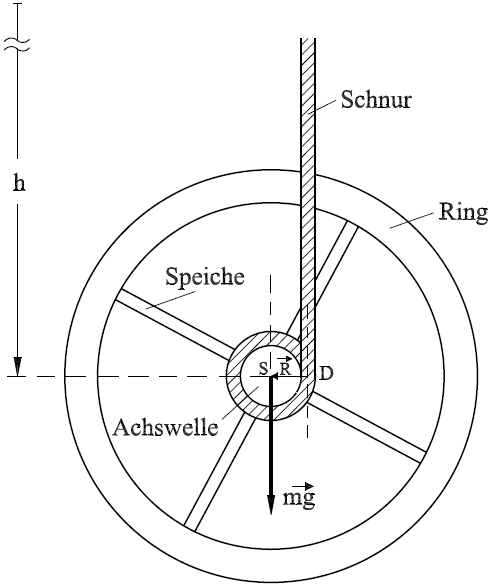
\includegraphics[width=0.5\textwidth]{fallrad}
  \caption{Maxwellsches Fallrad \footcite{anleitung-ws2014}}
  \label{fig:fallrad}
\end{figure}
\begin{figure}[H] 
  \centering
	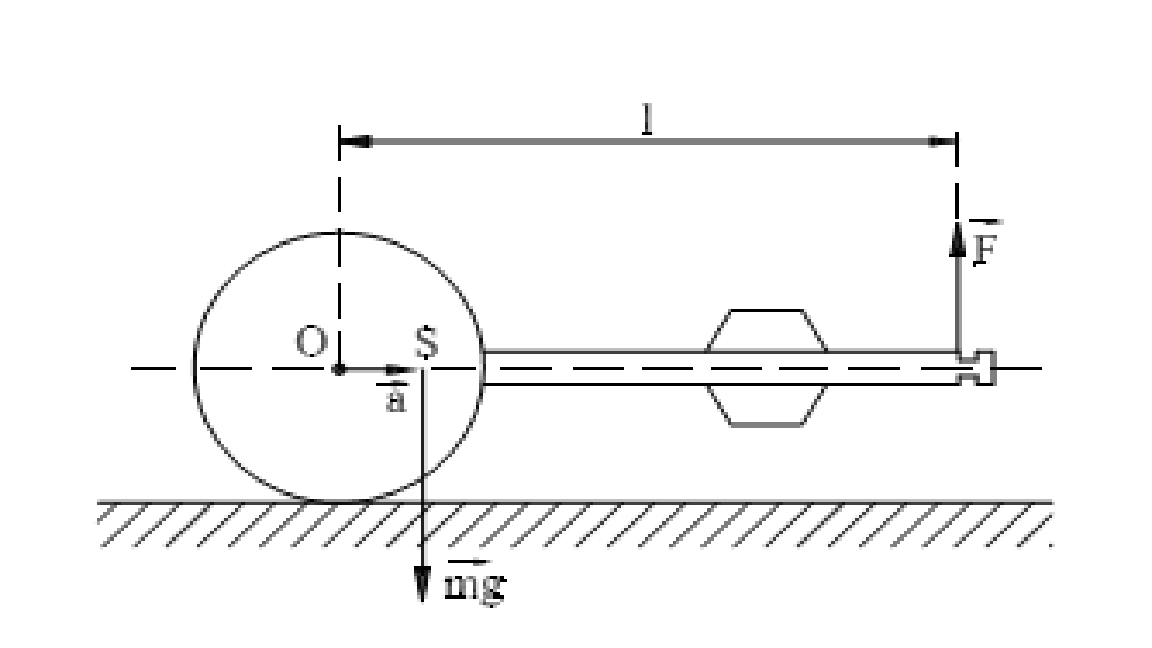
\includegraphics[width=0.7\textwidth]{abestimmung.png}
	\caption{Bestimmung der Größe $amg$}
  \label{fig:abestimmung}
\end{figure}
Die Dichte $\rho$ wird berechnet durch die Gesamtmasse $m$ und Volumen $V$ des Rades:
\begin{equation}
  \rho=\frac{m}{V}=\frac{m}{V_{\text{Ring}}+V_{\text{Achse}}+2V_{\text{Speiche}}}
  \label{eq:dichte}
\end{equation}
\subsection{Kreisel}
\section{Versuch M5: Maxwellsches Fallrad}
Ziel des Versuches ist die Bestimmung des Abrollradius $R$ durch Messung von Fallhöhe, Fallzeit und Berechnung des Trägheitsmomentes.
Zunächst wird ein senkrechter neben dem Fallrad stehender Maßstab so justiert, dass bei vollständiger Abwicklung der Schnur die 0 genau auf Höhe der Achse liegt.
Nun wird das Fallrad von 5 verschiedenen Höhen je 5 mal fallen gelassen und die Zeit vom Loslassen bis zum niedrigsten Punkt $h_{\text{max}}$ mit einer Stoppuhr gemessen.

Es wird aus der Theorie (\cref{eq:fallhoehe}) erwartet, dass die Fallzeit linear mit der Wurzel der Fallhöhe zusammenhängt.
\begin{table}[H]
  \centering
  \begin{tabular}{c | c | c | c | c | c | c}
    \diagbox{$h_{\text{max}}$}{$t$ [s]} & 1 & 2 & 3 & 4 & 5 & Mittelwert \\ \hline
    \SI{20}{cm} & \num{3.75} & \num{3.56} & \num{3.63} & \num{3.66} & \num{3.72} & \SI{3.66 \pm 0.08}{s} \\
    \SI{40}{cm} & \num{5.06} & \num{5.13} & \num{5.25} & \num{5.47} & \num{5.25} & \SI{5.23 \pm 0.16}{s} \\
    \SI{60}{cm} & \num{6.62} & \num{6.34} & \num{6.59} & \num{6.41} & \num{6.72} & \SI{6.54 \pm 0.16}{s} \\
    \SI{80}{cm} & \num{7.88} & \num{7.44} & \num{7.72} & \num{7.56} & \num{7.56} & \SI{7.63 \pm 0.17}{s} \\
    \SI{99}{cm} & \num{8.38} & \num{8.28} & \num{8.09} & \num{8.47} & \num{8.28} & \SI{8.30 \pm 0.14}{s} \\
  \end{tabular}
  \caption{Fallzeit $t$ bei verschiedenen Fallhöhen $h_{\text{max}}$}
  \label{tab:fallzeit}
\end{table}
Der geschätzte Fehler für die Höhenmessung beträgt jeweils $\SI{\pm 0.5}{cm}$, für die Zeitmessung $\SI{\pm 0.5}{s}$.
Bei der letzten Messung konnte nicht von \SI{100}{cm} Höhe gemessen werden, da das Fallrad an die Aufhängung stieß. \\

Wie erwartet steigt die Fallzeit mit zunehmender Höhe. Im ersten Diagramm wird eine Wurzelfunktion erwartet, das zweite sollte eine Gerade zeigen. Im dritten Diagramm erwarten wir aus \cref{eq:fallhoehe}, dass der Quotient $h_{\text{max}}/t^2=0.5g^*$ konstant, also unabhängig von der Fallzeit ist.

\begin{figure}[H]
  \centering
  \begin{tikzpicture}
    \begin{axis}[
      width=15 cm,
      height=9 cm,
      xmin=15, xmax=105,
      ymin=0, ymax=10,
      xlabel={Fallhöhe $h_{\text{max}}$ [cm]},
      ylabel={Fallzeit $t$ [s]}
    ]
      \addplot[mark=x, only marks, error bars/.cd, x dir=both, x fixed=0.5, y dir=both, y explicit] table[y error index=2] {ht.txt};
    \end{axis}
  \end{tikzpicture}
  \caption{Fallzeit $t$ in Abghängigkeit der Fallhöhe $h_{\text{max}}$}
  \label{fig:ht}
\end{figure}

\begin{figure}[H]
  \centering
  \begin{tikzpicture}
    \begin{axis}[
      width=15 cm,
      height=9 cm,
      xmin=15, xmax=105,
      ymin=10, ymax=75,
      xlabel={Fallhöhe $h_{\text{max}}$ [cm]},
      ylabel={Quadrat der Fallzeit $t^2$ [$s^2$]}
    ]
      \addplot[mark=x, only marks, error bars/.cd, x dir=both, x fixed=0.5, y dir=both, y explicit] table[y error index=2] {ht2.txt};
    \end{axis}
  \end{tikzpicture}
  \caption{Quadrat der Fallzeit $t^2$ in Abghängigkeit der Fallhöhe $h_{\text{max}}$}
  \label{fig:ht2}
\end{figure}
\begin{figure}[H]
  \centering
  \begin{tikzpicture}
    \begin{axis}[
      width=15 cm,
      height=9 cm,
      xmin=1, xmax=2,
      ymin=0, ymax=10,
      xlabel={$h_{\text{max}}/t^2$ [\si{cm/s^2}]},
      ylabel={Fallzeit $t$ [s]}
    ]
      \addplot[mark=x, only marks, error bars/.cd, x dir=both, x explicit, y dir=both, y explicit] table[x error index=2, y error index=3] {hdurchtgegent.txt};
    \end{axis}
  \end{tikzpicture}
  \caption{Fallzeit $t$ in Abghängigkeit von $h_{\text{max}}/t^2$}
  \label{fig:hdurchtgegent}
\end{figure}
Der Erwartung entsprechend streuen sich die Werte für $h_{\text{max}}/t^2$ innerhalb des Fehlers um einen Wert:
\begin{table}[H]
  \centering
  \begin{tabular}{c | c | c | c | c | c | c}
    & 1 & 2 & 3 & 4 & 5 & Mittelwert \\ \hline
    $h_{\text{max}}/t^2$ [\si{cm/s^2}] & \num{1.49} & \num{1.46} & \num{1.40} & \num{1.37} & \num{1.44} & \num{1.43\pm .05}
  \end{tabular}
  \caption{Werte für $h_{\text{max}}/t^2$}
  \label{tab:gstern}
\end{table}
Aufgrund des geringen relativen Fehlers von $\frac{0.05}{1.43}\approx\SI{3.5}{\percent}$ kann dieser (wie aus der Theorie erwartet) als konstant angenommen werden.
Für $g^*$ erhält man:
\begin{equation}
  g^*=\SI{2.87\pm .10}{cm/s^2}
  \label{eq:gsterngemessen}
\end{equation}
Um das Trägheitsmoment des Rades zu bestimmen, wurden nun die Maße des Ringes, der Speichen und der Achse mit einer Schieblehre gemessen. Da Unsicherheiten beim Innen- und Aussenradius $R_i$ bzw. $R_a$ besonders stark das Ergebnis beeinflussen (vgl. \cref{eq:traegheit_symmetrieachse}: 4. Potenz) und diese beim Ring am größten sind, wird jede Messung hier 5 mal an verschiedenen Stellen wiederholt.
\begin{table}[H]
  \centering
  \begin{tabular}{c | c | c}
    Dicke $H_R$ & Außenradius $R_a$ & Innenradius $R_i$ \\ \hline
    \SI{11.54\pm .24}{mm} & \SI{9.94\pm .07}{cm} & \SI{8.76}{cm}
  \end{tabular}
  \caption{Maße des Ringes}
  \label{tab:ringwerte}
\end{table}
Die Standardabweichung beim Innenradius liegt außerhalb der signifikaten Stellen.
Die anderen Maße wurden einmal gemessen und der Fehler geschätzt:
\begin{table}[H]
  \centering
  \begin{tabular}{c | c | c}
    Durchmesser d. Speiche $d_S$ & Länge d. Achse $H_A$ & Durchmesser d. Achse $d_A$ \\ \hline
    \SI{8.06\pm .05}{mm} & \SI{20.00\pm 0.02}{cm} & \SI{8.00\pm .05}{mm}
  \end{tabular}
  \caption{Maße von Speiche und Achse}
  \label{tab:speicheachse}
\end{table}
Die Gesamtmasse des Rades wird durch eine Waage bestimmt ($m=\SI{848.68\pm .01}{g}$) und die Dichte berechnet. Es wird näherungsweise dieselbe Dichte für alle Bestandteile des Rades angenommen:
\begin{align}
  V_{\text{Ring}}&=H_R\pi(R_a^2-R_i^2)=\SI{80.00\pm 5.32}{cm^3} \\
  V_{\text{Achse}}&=H_A\pi\left(\frac{d_A}{2}\right)^2=\SI{10.05\pm .25}{cm^3} \\
  V_{\text{Speiche}}&=2R_i\pi\left(\frac{d_S}{2}\right)^2=\SI{8.94\pm .22}{cm^3} \\
  \rho&=\frac{m}{V_{\text{Ring}}+V_{\text{Achse}}+2V_{\text{Speiche}}}=\SI{7.86\pm .39}{g/cm^3}
  \label{eq:dichte}
\end{align}
Es wird näherungsweise mit dem Innendurchmesser $2R_i$ des Ringes als Länge einer Speiche gerechnet, obwohl in der Realität die Achse in der Mitte die Speichen durchstößt. Dadurch kann die Rechnung von 4 auf 2 Speichenträgheitsmomente reduziert werden und Schwerpunkt von Speiche und Rad stimmen überein. Wir berechnen Trägheitsmomente von Ring und Achse bezüglich ihrer Symmetrieachse (\cref{eq:traegheit_symmetrieachse}) und von den Speichen senkrecht dazu (\cref{(eq:traegheit_senkrecht}):
\begin{table}[H]
  \centering
  \begin{tabular}{c | c | c}
    $J_{\text{Ring}}$ & $J_{\text{Achse}}$ & $J_{\text{Speiche}}$ \\ \hline
    \SI{5.52\pm .49}{g.m^2} & \SI{6.32\pm .35}{g.cm^2} & \SI{0.184\pm .009}{g.m^2}
  \end{tabular}
  \caption{Trägheitsmomente}
  \label{tab:traegheit_berechnet}
\end{table}
Insgesamt haben wir für das Trägheitsmoment des Rades:
\begin{equation}
  J_S=J_{\text{Ring}}+J_{\text{Achse}}+2J_{\text{Speiche}}=\SI{5.89\pm .49}{g.m^2}
  \label{eq:traegheitgesamt}
\end{equation}
Die relative Unsicherheit beträgt $\frac{0.49}{5.89}\approx \SI{8.3}{\percent}$. Im Verhältnis gesehen zu den vielen Messwerten, die an der Berechnung beteiligt sind, ist diese Unsicherheit gering und es lässt sich mit dem Wert gut weiterarbeiten.

\cref{eq:fallhoehe} wird umgestellt, um $R$ zu berechnen:
\begin{equation}
  R=\sqrt{\frac{J_S\cdot g^*}{m(g-g^*)}}=\SI{4.51\pm .20}{mm}
  \label{eq:abrollradius}
\end{equation}
Auch hier ist die relative Unsicherheit mit $\frac{0.20}{4.51}\approx \SI{4.4}{\percent}$ sehr gering. Bei der Probe durch Vergleich mit den direkt über die Schieblehre gemessenen Längen wird eine gute Übereinstimmung erwartet.
Dazu wurde die Dicke der Schnur an 5 verschiedenen Stellen gemessen: $d_S=\SI{1\pm0.05}{mm}$. Da jedesmal derselbe Wert gemessen wurde, wird die Dicke der Schnur über die gesamte Länge als konstant angenommen. Der Durchmesser der Achse $d_A$ wird aus \cref{tab:speicheachse} übernommen und der Vergleichswert $R_{\text{direkt}}$ errechnet:
\begin{equation}
  R_{\text{direkt}}=\frac{1}{2}(d_A+d_D)=\SI{4.50\pm .04}{mm}
  \label{eq:vergleichswert}
\end{equation}
Wir haben also eine absolute Abweichung von $R-R_{\text{direkt}}=\SI{.01}{mm}$ und eine relative Abweichung von nur \SI{.2}{\percent}.
\section{Versuch M6: Kreisel}
Der gemessene Kreisel besteht aus einer Kugel der Masse $m_k= 512,38 \pm 0,01g$ und dem Durchmesser $d_k=50,70 \pm 0,05 mm$ und einem Stab der Länge $L=(84,65\pm 0,05 mm)$ mit einem Zusatzgewicht (vgl. Abbildung~\ref{fig:abestimmung})
\subsection{Experimentelle Bestimmung von $J_k$}
\subsubsection{Bestimmung von $\vec a$}
Die Bestimmung des Abstandes $a$ zwischen dem Schwerpunkt $S$ und Unterstützpunkt $O$ erfolgt indirekt, in dem die Kraft $F$ und die Länge $l = (110 \pm 0,05mm)$ aus der Abbildung~\ref{fig:abestimmung} bestimmt werden. Während sich $l$ aus der Summe der Länge der Stange $L$ und des Radius der Kugel $r_k=(25,35\pm 0,05mm)$ ergibt, wird $F$ mit Hilfe eines Kraftmessers für die einzelnen Positionen des Zusatzgewichts bestimmt.
\begin{table}[H]
  \centering
  \begin{tabular}{c | c | c | c | c | c | c}
    \diagbox{\small{Position}}{Messung} & 1 & 2 & 3 & 4 & 5 & Mittelwert \\ \hline
    1 & $0,12$ N &  $0,11$ N & $0,11$ N & $0,13$ N & $0,12$ N &  $(0,12\pm0,01)$ N \\
    2 & $0,13$ N &  $0,17$ N & $0,18$ N & $0,17$ N & $0,17$ N &  $(0,17\pm0,01)$ N \\
    3 & $0,23$ N &  $0,22$ N & $0,22$ N & $0,23$ N & $0,22$ N &  $(0,22\pm0,01)$ N 
  \end{tabular}
  \caption{Die Kraft $F$ für die unterschiedlichen Stelllungen der Zusatzmassen}
  \label{tab:Fpositionen}
\end{table}
Bei der Messung wurden alle Messwerte mit einem geschätztem Fehler von $\Delta F=\pm 0,01N$ bestimmt.
Position 1 ist erreicht, wenn sich das Zusatzgewicht direkt an der Kugel befindet, Position 3, wenn es sich direkt an der Kerbe, an der $F$ bestimmt wird, befindet, und Position 2 mittig.
\subsubsection{Bestimmung der Präzessionszeit $T_p$}
Die Bestimmung der Präzessionszeit $T_p$ erfolgt bei unterschiedliche Positionen des Zusatzgewichts und unterschiedlichen Frequenzen des Kreisels. Dafür wird mit Hilfe von einer Pressluft und einem Stroboskop $\omega$ möglichst konstant gehalten und $T_p$ mit Hilfe einer Stoppuhr bestimmt. Um den Messfehler dabei möglichst gering zu halten, wird die Präzessionszeit für insgesamt fünf Umdrehungen bestimmt und anschließend über diese Werte gemittelt.

\begin{table}[H]
  \centering
  \begin{tabular}{c | c | c | c}
    Zusatzgewicht- & Frequenz f in& $\omega$ in &$T_p$ in\\
    position & Hz $(\pm 1 Hz)$ &  $s^{-1}\pm 5 s^{-1}$ & s$(\pm 0,5 s)$\\ \hline
      & \num{18,3} & \num {115,0} & \num{7,3}\\
      & \num{25} & \num {157,1}& \num{9,9}\\
    1 & \num{31,6} & \num {198,6} & \num{12,7}\\
      & \num{40} & \num {251,3}& \num{15,8}\\
      & \num{50} & \num {314,2}&\num{19,4}\\ \hline
      & \num{18,3} & \num {115,0}& \num{4,8}\\
      & \num{25} & \num {157,1}& \num{6,6}\\
    2 & \num{31,6} & \num {198,6}& \num{8,3}\\
      & \num{40} & \num {251,3}& \num{10,5}\\
      & \num{50} & \num {314,2}& \num{12,9}\\ \hline
      & \num{18,3} & \num {115,0}& \num{3,7}\\
      & \num{25} & \num {157,1}& \num{5,1}\\
    3 & \num{31,6} & \num {198,6}& \num{6,5}\\
      & \num{40} & \num {251,3}& \num{8,2}\\
      & \num{50} & \num {314,2}& \num{10,2}\\ 
  \end{tabular}
  \caption{Präzessionszeit des Kreisels in Abhängigkeit von f und der Position des Gewichts}
  \label{tab:Präzezeit}
\end{table}

\begin{figure}[H]
  \centering
  \begin{tikzpicture}[domain=60:320]
    \begin{axis}[
      width=15 cm,
      height=9 cm,
      xmin=0, xmax=330,
      ymin=0, ymax=25,
      xlabel={Eigenfrequenz},
      ylabel={Präzessionzeit Tp [s]}
    ]
     \addplot[mark=x, only marks, error bars/.cd, y dir=both, y fixed=0.5, x dir=both, x fixed=0.5] table {pos1.txt};
     \addplot+[mark=none] {0.062*x};
    \end{axis}
  \end{tikzpicture}
  \caption{Präzessionzeit mit Gewicht in Position 1}
  \label{fig:pos1}
\end{figure}

\begin{figure}[H]
  \centering
  \begin{tikzpicture}[domain=60:320]
    \begin{axis}[
      width=15 cm,
      height=9 cm,
      xmin=0, xmax=330,
      ymin=0, ymax=20,
      xlabel={Eigenfrequenz},
      ylabel={Präzessionzeit Tp [s]}
    ]
     \addplot[mark=x, only marks, error bars/.cd, y dir=both, y fixed=0.5, x dir=both, x fixed=0.5] table {pos2.txt};
     \addplot+[mark=none] {0.042*x};
    \end{axis}
  \end{tikzpicture}
  \caption{Präzessionzeit mit Gewicht in Position 2}
  \label{fig:pos1}
\end{figure}

\begin{figure}[H]
  \centering
  \begin{tikzpicture}[domain=60:320]
    \begin{axis}[
      width=15 cm,
      height=9 cm,
      xmin=0, xmax=330,
      ymin=0, ymax=15,
      xlabel={Eigenfrequenz},
      ylabel={Präzessionzeit Tp [s]}
    ]
     \addplot[mark=x, only marks, error bars/.cd, y dir=both, y fixed=0.5, x dir=both, x fixed=0.5] table {pos3.txt};
      \addplot+[mark=none] {0.033*x};
    \end{axis}
  \end{tikzpicture}
  \caption{Präzessionzeit mit Gewicht in Position 3}
  \label{fig:pos1}
\end{figure}

In sämtlichen Diagrammen sind die Fehler der Eigenfrequenz aufgrund ihrer relativ geringen Größe nicht genau eingetragen. Und die mit \emph{gnuplot} entwickelten Funktionen sind jeweils dazu eingetragen.


Mit \emph{gnuplot} werden nach dem \emph{least-squares}-Verfahren die Werte gegen die Funktion $f(x)=k\cdot x$ gefittet. Ausgabe:

\begin{table}[H]
  \centering
  \begin{tabular}{c | c | c}
    Gewichtsposition & Wert für $k$ & Varianz der Residuen \\ \hline
    1 & $k_1=\num{0,062\pm 0,00041}$ & \num{0,04} \\
    2 & $k_2=\num{0,042\pm0,00019}$ & \num{0,008}\\
    3 & $k_3=\num{0,033\pm 0,00006}$ & \num{0,001}\\
  \end{tabular}
  \caption{Linearer Fit der Präzessionszeit}
  \label{tab:präzefit}
\end{table}

\begin{table}[H]
  \centering
  \begin{tabular}{c | c | c | c}
    Gewichtsposition & Wert für $k$ & Inverses von $k$ & $lF$ in $cm\cdot mN$ \\ \hline
    1 & $k_1=\num{0,062\pm 0,00041}$ & \num{16,13\pm 0,11} & \num{1320 \pm 110}\\
    2 & $k_2=\num{0,042\pm0,00019}$ & \num{23,81\pm 0,11} & \num{1870 \pm 110}\\
    3 & $k_3=\num{0,033\pm 0,00006}$ & \num{30,30 \pm 0,06} & \num{2420 \pm 110}\\
  \end{tabular}
  \caption{Linearer Fit der Präzessionszeit}
  \label{tab:präzefit}
\end{table}
Der Fehler des Produkt 
\begin{equation}
\Delta (lF)= \sqrt{(l\Delta F)^2+(F \Delta l)^2}=110,
\end{equation}
und des Kehrwerts
\begin{equation}
\Delta \frac{1}{k}=\frac{1}{k^2}\Delta k
\end{equation}
ergeben sich nach der Fehlerfortpflanzung

\begin{figure}[H]
  \centering
  \begin{tikzpicture}[domain=16:31]
    \begin{axis}[
      width=15 cm,
      height=9 cm,
      xmin=0, xmax=35,
      ymin=0, ymax=2500,
      xlabel={Kehrwert der Steigung},
      ylabel={lF in $cm\cdot mN$}
    ]
     \addplot[mark=x, only marks, error bars/.cd, y dir=both, y fixed=110, x dir=both, x fixed=0.5] table {lfgegens.txt};
      \addplot+[mark=none] {79.7293*x};
    \end{axis}
  \end{tikzpicture}
  \caption{lF gegen den Kehrwert der Steigungen k}
  \label{fig:pos1}
\end{figure}
Mit \emph{gnuplot} werden nach dem \emph{least-squares}-Verfahren die Werte gegen die Funktion $f(x)=s\cdot x$ gefittet. Ausgabe:
\begin{table}[H]
  \centering
  \begin{tabular}{c | c}
     Wert für $s$ & Varianz der Residuen \\ \hline
     $(7972,93\pm 75,23)gcm^2$ & \num{987.68} 
  \end{tabular}
  \caption{Linearer Fit von lF gegen den Kehrwert von k}
  \label{tab:präzefit}
\end{table}

Daraus folgt für das Trägheitsmoment
\begin{equation}
J_K=\frac{s}{2\pi}=(1268,93\pm 12)gcm^2
\end{equation}

\subsubsection{Mathematische Bestimmung von $J_K$}
Der Kreisel besteht nur aus einer Kugel und einem Stab, dessen Trägheitsmoment $J_1=15gcm^2$ bekannt ist. Deswegen ergibt sich das Trägheitsmoment aus der Summe der beiden Objekten.
\begin{gather}
J_{ges}=J_{Kugel}+J_{Stab}
= \frac{2}{5} m r^2 + J_{Stab}\\
J_{ges}= (1332,07\pm 2,60)gcm^2
\end{gather}
\section{Abschließende Diskussion}
Beim Versuch zum Maxwellschen Fallrad wurde der Abrollradius bestimmt:
\begin{equation}
  R=\SI{4.51\pm0.20}{mm}
  \label{eq:abrollradius_wiederholt}
\end{equation}
Es gab einige mögliche Fehlerquellen:
\begin{itemize}
  \item Es war schwierig, das Rad gleichzeitig an beiden Enden loszulassen. Besonders bei größeren Höhen konnte das Rad leicht ins trudeln kommen, was möglicherweise die Fallzeit verfälscht
  \item Die Reaktionszeit des Zeitstoppenden erhöht die Unsicherheit der Zeitmessung
  \item Beim Messen des Innen-und Außenradiusses war die Achse der Schieblehre im Weg
  \item Die Buchse in der Mitte des Rades wurde vernachlässigt. Außerdem wurde mit 2 Speichen gerechnet, die durch die Mitte hindurchführen, anstatt mit 4 kleineren Speichen, die nur bis zur Achse reichen.
\end{itemize}
Von diesen Fehlerquellen schätzen wir die Reaktionszeit beim Zeitstoppen als die signifikanteste ein. \\

Trotz der Fehlerquellen wurde ein außerordentlich genaues Ergebnis erziehlt. sowohl was die relative Unsicherheit von nur \SI{4.4}{\percent} angeht, als auch beim Vergleich mit dem direkt gemessenen Wert: Hier betrug die relative Abweichung nur \SI{0.2}{\percent}.

Grund dafür könnte sein, dass die Fehler durch mehrfaches Messen und anschließende Mittelwertbildung minimiert wurde: Zur Bestimmung von $h_{\text{max}}$ gab es je 5 Messungen bei 5 verschiedenen Höhen, insgesamt also 25 Datenpunkte, sodass der statistische Fehler gering wurde.
Auch der Innen-und Außenradius $R_i$ bzw. $R_a$ des Ringes, der mit 4. Potenz in das Trägheitsmoment des Rades eingeht (\cref{eq:traegheit_symmetrieachse}), wurde je 5 mal gemessen. 

Aus dem sehr genauen Ergebnis schließen wir
\begin{enumerate}
  \item Der Zusammenhang zwischen Fallhöhe und Fallzeit $h(t)$ aus der Theorie (\cref{eq:fallhoehe}) ist bestätigt. Das Fallrad erfährt eine konstante Beschleunigung $g^*$, die sich aus dem Trägheitsmoment, der Masse und dem Abrollradius des Rades zusammensetzt
  \item Es lohnt sich, vor der Messung den Einfluss von Messwerten und -unsicherheiten auf das Endergebnis abzuschätzen und gegebenenfalls längere Messreihen durchzuführen, um den Fehler zu minimieren
\end{enumerate}

\nocite{anleitung-ws2014}
